%\documentclass[10pt,a4paper]{article}

\documentclass[24pt]{article}

\usepackage{arxiv}
\usepackage[utf8]{inputenc} % allow utf-8 input
\usepackage[T1]{fontenc}    % use 8-bit T1 fonts
\usepackage{hyperref}       % hyperlinks
\usepackage{url}            % simple URL typesetting
%\usepackage{booktabs}       % professional-quality tables
\usepackage{amsfonts}       % blackboard math symbols
\usepackage{nicefrac}       % compact symbols for 1/2, etc.
\usepackage{microtype}      % microtypography
\usepackage{lipsum}         % Can be removed after putting your text content
\usepackage{graphicx}
\usepackage{natbib}
\usepackage{doi}
\usepackage{amssymb}
\usepackage{amsthm}
\usepackage{forest}


\usepackage{tikz} 
\usepackage{caption}
\usepackage{amsmath}
\usepackage{cleveref}       % smart cross-referencing
\usepackage{colortbl}
\usepackage{color}
\usepackage{listings}
\usepackage{multicol}
\usepackage{array}

\definecolor{orange151}{rgb}{0.9,0.647,0}
\definecolor{lgreen}{rgb}{0.564,0.93,0.564}


\usepackage{color}

\definecolor{dkgreen}{rgb}{0,0.6,0}
\definecolor{gray}{rgb}{0.5,0.5,0.5}
\definecolor{mauve}{rgb}{0.58,0,0.82}

\lstset{frame=none,
  language=Python,
  aboveskip=3mm,
  belowskip=3mm,
  showstringspaces=false,
  columns=flexible,
  basicstyle={\small\ttfamily},
  numbers=none,
  numberstyle=\tiny\color{gray},
  keywordstyle=\color{blue},
  commentstyle=\color{dkgreen},
  stringstyle=\color{mauve},
  breaklines=true,
  breakatwhitespace=true,
  tabsize=3
}
\definecolor{dgreen}{rgb}{0,0.5,0}
\definecolor{bg}{rgb}{0.125,0.51,0.49}
\definecolor{mag}{rgb}{0.866,0.627,0.866}
\definecolor{lgray}{rgb}{0.49,0.49,0.49}
\definecolor{dgray}{rgb}{0.82,0.788,0.827}
\definecolor{pink}{rgb}{1, 0.568, 0.686}
\definecolor{lblue}{rgb}{0.078, 0.741, 0.931}
\definecolor{orag2}{rgb}{0.87, 0.478, 0.12}

\newcommand*{\addheight}[2][.5ex]{%
  \raisebox{0pt}[\dimexpr\height+(#1)\relax]{#2}%
}

%\newcommand{\subf}[2]{%
%  {\small\begin{tabular}[t]{@{}c@{}}
%  #1\\#2
%  \end{tabular}}%
%}

\newtheorem{theorem}{Theorem}[section]
\newtheorem{lemma}[theorem]{Lemma}
\newtheorem{proposition}[theorem]{Proposition}
\newtheorem{corollary}[theorem]{Corollary}
\newtheorem{example}[theorem]{Example}
\newtheorem{definition}[theorem]{Definition}


\title{Snakes}

%\author{ \href{https://orcid.org/0000-0002-8749-3324}{
\includegraphics[scale=0.08]{orcid.pdf} \href{mailto: jacques.bourg739@gmail.com}{@}\hspace{1mm} Jacques Bourg    }}
\author{Jacques Bourg}


% Uncomment to override  the `A preprint' in the header
\renewcommand{\headeright}{}
\renewcommand{\undertitle}{}
\renewcommand{\shorttitle}{Snakes}


\hypersetup{
pdftitle={Snakes}, 
pdfsubject={math.NT},
pdfauthor={Jacques Bourg},
pdfkeywords={Snakes, active contours, contour models, object tracking, shape recognition, segmentation, edge detection. },
}
 

\begin{document}

\maketitle

\begin{abstract}

I go in detail over how does a snake works. I also present my own implementation of the Snakes. 
\end{abstract}

\keywords{Snakes, active contours, contour models, object tracking, shape recognition, segmentation, edge detection.}



\section{Snakes}

As defined in the original paper      \cite{Snake}  by 
 Kass,  Witkin, and Terzopoulos, a snake is an "energy-minimizing
spline guided by external constraint forces and influenced by image
forces that pull it toward features such as lines and edges. Snakes are active contour models: they lock
onto nearby edges, localizing them accurately."


To expand, we want to isolate precisely the boundaries of an object, starting from a rough encirclement of it. The snake model will iteratively move the contour to fit precisely the object boundary.  

We say that the contour is active since it is iteratively warped in order to approach the pixels with higher gradient. Also as we will how to add a shape constraint to the snake in order to enforce smoothness.

There are three main parts in the algorithm:  initialization, deformation and convergence. The algorithm converges when the total movement is small from one iteration to the other.  


Snakes have several applications. For instance, they can be used to track objects over time, the snake at one frame serving as initial contour of the next frame. 






\section{Theory}

As said in the paper, the active contour introduced a variational approach consisting in minimizing an energy functional.  Before this idea, the traditional approach in computer vision was to detecting edges and linking them afterwards. The snake energy can be decomposed as having three terms: an image term a smoothness term and an elastic term, and can be integrated along the contour.


$$E_{snake} = E_{image} + \alpha.E_{elastic} + \beta.E_{smooth}= \int_0^1  E_{image}(s)  + \alpha.E_{elastic}(s) + \beta.E_{smooth}(s) .ds $$ 


The snake is sampled at what we call control points. Be interpolate straigth segments between control points. The Snake energy is evaluated at control points: $\{cp_i\}_{i \in [1, N_{cp}]}$. 


$$E_{snake} = \sum_{i= 1}^{N_{cp}} E_{snake}(cp_i) = \sum_{i= 0}^{N_{cp}-1} E_{snake}(cp_i) $$


Setting an arbitrary point along the snake contour as origin, the curvilinear coordinate along the contour is noted $s$. The position of a contour point $p$ has a curvilinear coordinate $s$ and coordinates in the canonical base $p = \begin{bmatrix}
  x \\
  y
\end{bmatrix}$. 




\subsection{Image energy}

	Convolving a Gaussian of a certain width with an image and then 
computing the norm of the gradient, creates a scalar field near the edges of the image.  We define $ G = || \nabla (n_{\sigma} * I) || $ as the gradient of the image convolved by the Gaussian kernel. G has the same dimensions of the image $I$. 

Therefore, a control point that can sense non nil regions of the gradient G within a window centered on himself, will be able to move locally to a point of higher image energy, in order to \textbf{maximize}  the image energy of the snake. 



The image energy term is computed as:

$$E_{image} = \sum_{i = 0}^{N_{cp}-1} G_{(x_i, y_i)} $$ where $(x_i,y_i)$ are the coordinates of the control points  
 
\subsection{Elastic energy} 
   The elastic energy of a contour is the sum over the control points of the squares of the position derivatives:
   
   $$E_{elastic} = || \frac{dp}{ds}||^2 = \sum_{n_{cp} = -1}^{N_{cp}-1} ||p_{n_{cp}+1} -  p_{n_{cp}} ||  = \sum_{n_{cp} = -1}^{N_{cp}-1} (x_{i+1} - x_{i})^2 + (y_{i+1} - y_{i})^2   $$   

I adopt the notation $\sum_{i = -1}^{N_{cp}-1} $ to account for the fact that, as the contour is a polygon, we have to take into account the link between the last contour point and the first one. 

\subsection{Smooth energy} 

 The smooth energy of a contour is the sum over the control points of the squares of the second derivatives:
   
   $$E_{smooth} = || \frac{d^2p}{ds^2}||^2  = \sum_{n_{cp} = -1}^{N_{cp}-1} (x_{i+1} - 2 x_{i} + x_{i-1})^2 + (y_{i+1} - 2 y_{i} + y_{i-1})^2   $$   

The both the elastic energy as well as the smooth energy have to be \textbf{minimized}. Then, we will redefine the image energy as $E_{image} \leftarrow -E_{image}$ so that all the three energies are minimized together. 

\subsection{Local minimization of the energy} 

In the following figure, we can have an idea of how does the energy minimization happens. Control points are black points. At iteration n, we center a grid around a control point and evaluate the snake energy considering all the points of the grid, and choosing as next point, the point with minimal energy. 


The image energy is computed in the following way: it corresponds to minus the gradient G of the image in every point of the grid, and in  the resting positions of of the control points. 

The smooth and elastic energy terms are computed, for every pixel, by creating a list of positions of $\textbf{all}$ the control points which include the position of the point of the grid being tested. Therefore each $\textbf{shape}$ of the snake has a smooth and an elastic energy associated with it.  
 


\begin{figure}[h!]
  \centering
  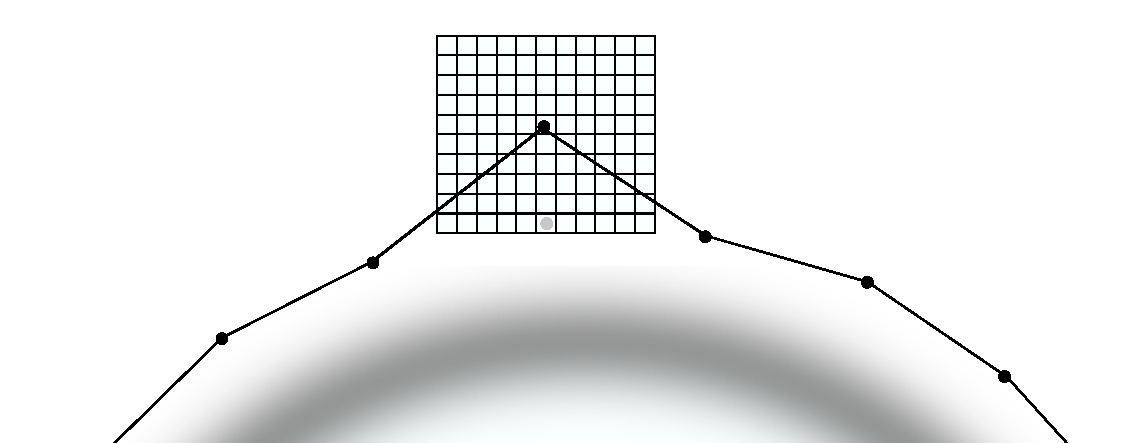
\includegraphics[width=0.8\textwidth]{minimisation.pdf}
  \caption{Energy minimization of the snake. We evaluate the $E_{snake}$ energy on a grid centered on the actual position of a control point. The gray point is the candidate with higher gradient and lower $E_{smooth}$  and $E_{elastic}$.}
  \label{fig:en_min}
\end{figure}


\newpage

\subsection{Algorithms}


\subsection{Global algorithm}


Initial parameters:


$\Omega_{W_h}$: Square window (of  half size $W_h$) around each control point,  on which will be evaluated the snake energy function. 

$\Theta$: (float) Motion threshold.
 
$N_{cp}$: (int) number of control points.
 
$\alpha, \beta$: (floats) weights of    
elastic  and smooth energy terms, knowing that $E_{snake} = E_{image} + \alpha.E_{elastic} + \beta.E_{smooth}$ 

$continue\_snake$ = True


$While$ $continue\_snake$:

~~~~	$For~ each~ control ~point~ i$:
	
~~~~~~~~	$(x',y') \leftarrow  min_{\Omega_{W_h}}( E_{snake}^{~~~~(x_i,y_i)} ) $


~~~~	$motion \leftarrow Compute ~total~motion (\{(x'_i,y'_i)_{i \in [0, N_c -1]} \})$

~~~~    $update ~contour()$

~~~~	if $motion >  \Theta$:

~~~~~~~~ $continue\_snake$ = False

~~~~    else:

~~~~~~~~ $resample\_contour()$


\subsection{Resample contour}
The resampling is a fundamental part for the algorithm convergence after each iteration. It consists of recreating equally spaced control points along the contour. We call $d(A,B)$ the euclidean distance between points $A$ and $B$: $d = \sqrt{(x_A-x_B)^2 + (y_A - y_B)^2}$.

Initial variables:

	- $\{cp'_i\}_{i= 1:N_{cp'}}$ : list of the newly computed positions $(x',y')$.

-$S_{total} = \sum_{i= -1}^{N_{cp'}}  ~~d(cp'_i , cp'_{i+1})$



- $s_{list} = \{j \frac{S_{total}}{N_{cp'}} \}_{j \in [0,1, ...N_{cp'}]} $

- $List ~contour~ =~ [~]$

for s $\in$ $s_{list}$:

~~~~~ for $cp_i$ $\in$ $\{cp'_i\}_{i= 1:N_{cp'}}$: 

~~~~~~~~~~ if $s_{(cp_{i})} \leq s$  and $s < s_{(cp_{i+1})} :$

~~~~~~~~~~~~~~~$(x'', y'') \leftarrow Interpolate ~coordinates ((x',y')^{(cp_{i})}, (x',y')^{(cp_{i+1})} , s  )$

~~~~~~~~~~~~~~~ $List ~contour += control\_point(x'', y'')$

     
\subsection{Interpolate coordinates}
	When an item $s$ of the new list of curvilinear coordinates is between the curvilinear coordinates of the new computed positions of two control points a and b, we need to create a new control point in the linear segment joining a and b. 
	
	
$$ x'' =  (s-s_a)\frac{x_b - x_a}{\sqrt{ (x_b - x_a)^2 + (y_b - y_a)^2 ))  } } + x_a    $$	
	
$$ y'' =  (s-s_a)\frac{y_b - y_a}{\sqrt{ (x_b - x_a)^2 + (y_b - y_a)^2 ))  } } + y_a    $$		
	
\subsection{Compute motion}

The displacement of the contour $\mu$ between an iteration and the next one can be computed, over all control points, as: 

$$ \mu = \sum_{i = 1}^{N_{cp}} d(cp_i , cp'_{i}) $$ 




\subsection{Clamp coordinates}
It happens, specially without regularisation terms $\alpha$ and $\beta$, that there are control points that wander around and that can even hit the border of the image. In that case, to avoid bugging the snake one can clamp the coordinates. For an image of dimensions $(L_y, L_x)$: 

 $$ x' = min\Big(max(W_h, x'), L_x - W_h \Big)  $$ 


 $$ y' = min\Big(max(W_h, y'), L_y - W_h \Big)  $$  
 
For each iteration of the snake, we clamp the coordinates twice:  

- Before computing the image energy term (which involves accessing grad, the gradient of the image convolved with a gaussian kernel). 
 
 \begin{lstlisting}
x,y = clamp_coordinates(x,y, W, (Ly, Lx))
win = grad[y - W: y + W+1, x - W: x + W + 1]
\end{lstlisting}

After having updated the coordinates:

 \begin{lstlisting}
 y_new = y - dy
 x_new = x - dx
 x_new,y_new = clamp_coordinates(x_new,y_new, W, (Ly, Lx))
 \end{lstlisting}

 

\subsection{Energy minimization} 




In the implementation, I made the choice of computing the next position  for each control point, but to do not update, in the same iteration the snake contour.   This make sense if you think about a snake that a given iteration n is a circle of diameter $d_1$ and at iteration n+1 is a circle of diameter $d_2$, $d_2 < d_1$.
When we do not update the control points just after having visited all of them makes that each of the control points at diameter n see the same vector field.





$E_{image}:$

~~~~ for $cp_i$ $\in$ $\{cp'_i\}_{i= 1:N_{cp'}}$:  
	
~~~~~~~~ $x_i$, $y_i$ = $x_{(cp_i)}$, $y_{(cp_i)}$

~~~~~~~~ $x_i$, $y_i$ $=  ~Clamp~ coordinates(x_i, y_i)$

~~~~~~~~ $W = G[y_i - W_h: y_i + W_h+1, x_i - W_h: x + W_h + 1]$

~~~~~~~~~~~~ for $cp_j$ $\in$ $\{cp'_i\}_{i= 1:N_{cp'}}$:

~~~~~~~~~~~~~~~~ $x_j$, $y_j$ = $x_{(cp_j)}$, $y_{(cp_j)}$

~~~~~~~~~~~~~~~~~~~~ if  $j \neq i$:

~~~~~~~~~~~~~~~~~~~~~~~~ $W \leftarrow W + G(x_j, y_j)$

$$ $$ 

$E_{elastic}~ \text{and}~ E_{smooth}:$
             
$E_{elastic} = zeros(shape(wind))$, $E_{smooth}  = zeros(shape(wind))$

       
$x\_arr =  x - W_h : x + W_h + 1$       

$y\_arr =  y - W_h : y + W_h + 1$ 

$ X, Y  = meshgrid(x\_arr, y\_arr) $  
                
for $ind\_y$, row in enumerate(X):

~~~~ for $ind\_x$, $\_$ $\in$
 enumerate(row):          
       
~~~~~~~~       $x\_arr\_temp = x\_arr.copy()$   
       
~~~~~~~~       $y\_arr\_temp = x\_arr.copy()$   
       
~~~~~~~~	   $Compute ~E_{elastic}[ x\_arr\_temp, y\_arr\_temp]$ 
	   
~~~~~~~~ 	   $Compute ~ E_{smooth}[ x\_arr\_temp, y\_arr\_temp]$ 

$y\_min, x\_min =  argmin(-W + \alpha E_{elastic} + \beta E_{smooth})$

$dy \leftarrow W_h - y\_min            $

$dx \leftarrow W_h - x\_min            $

$x' \leftarrow W_h  - x\_min$   
    
$y' \leftarrow W_h  - y\_min$   
   
$x', y' = clamp\_coordinates(x', y', W_h, (L_y, L_x))$
   
   
   
   






\newpage
 

\section{Implementation}
 
In the next section, I explain how I implemented the Snakes in Python. 

\subsection{Image gradient}

The original image was filtered with a gaussian kernel of standard deviation $\sigma = 15$, and the gradient was computed using the sobel filter from skimage. 

\begin{lstlisting}
gauss_filt = gaussian(im, sigma=15);
edges = filters.sobel(gauss_filt);
\end{lstlisting}


\begin{figure}[h!]
  \centering
  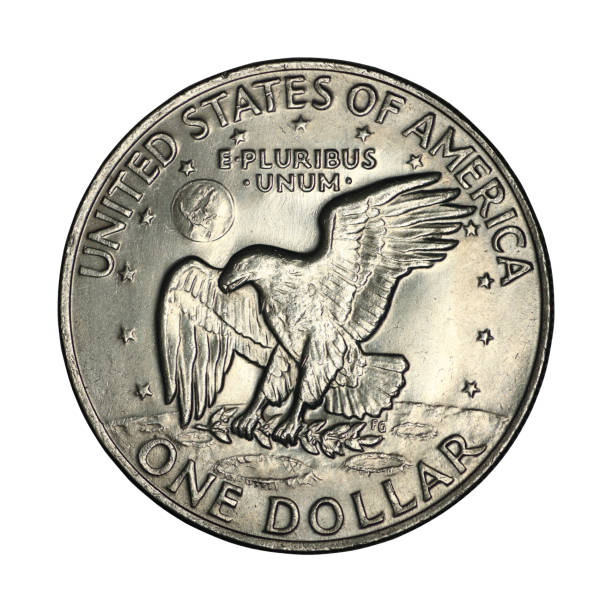
\includegraphics[width=0.2\textwidth]{Dollar.jpg}
  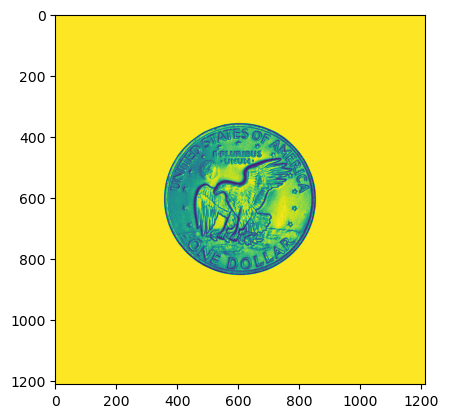
\includegraphics[width=0.23\textwidth]{coin.png}
  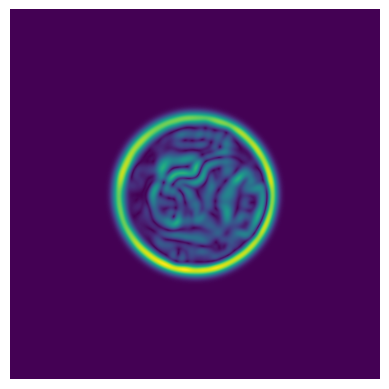
\includegraphics[width=0.20\textwidth]{grad.png}
  \caption{Left: original image. Center: padded and grayscaled image. Right: Gradient of the image.  }
  \label{fig:image_and_grad}
\end{figure}




\subsection{Control points}

A control point is declared as a class with the following instance attributes: $\textbf{x}$ and $\textbf{y}$ (integers), are the coordinates of one control point in the image. We create an initial contour that roughly surrounds the object to delineate, by creating a list of control points that follow the initial contour in order. We choose arbitrarily one of those control points as the origin of the contour. We assign a curvilinear coordinate  $\textbf{s}$ (a float) to each control point, that marks the piece-wise distance between the origin control point and the actual control point, passing by all the intermediary control points in straight segments. We initially declare s as None for each control point. We also declare two additional instance attributes for a control point  $\textbf{x\_prime}$ and $\textbf{y\_prime}$ (integers), initially instantiated as None, these coordinates are going to store the computed position of the control point at the next iteration. 



\subsection{Contours}

A contour is a class, whose most significant instance attribute  $\textbf{list\_change\_points}$  is a list containing the control points. 
At the initialization of a contour, it sets to zero the curvilinear coordinate of the first control point, and compute the curvilinear coordinate of all the others thanks to the method $\textbf{compute\_s()}$.

\begin{figure}[h!]
  \centering
  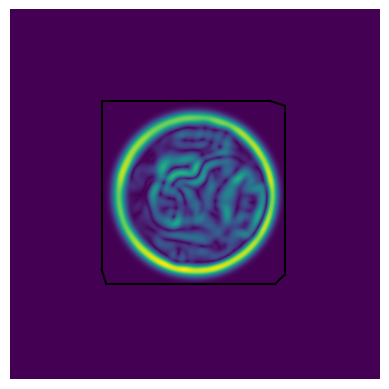
\includegraphics[width=0.2\textwidth]{control_point.png}
  \caption{Initialization of the snake using 40 control points.  }
  \label{fig:image_and_grad}
\end{figure}





\subsection{Shape energy terms}

 There is an optimization that made all the difference in the running time between iterations. By optimizing the code of the computation of the shape energy terms, I passed from around 5 minutes per iteration to less than a second. 
Instead of using a for loop I did the following:

Input parameters, two list of ordererd x and y coordinates:  $\{(x_i) \}_{i = 1,..., N_{cp}}$ and $\{(y_i) \}_{i = 1,..., N_{cp}}$. 


Add the last control point at the beginning of those lists:  $x\_array = \{x_{N_{cp}} \} U \{x_i \}_{i = 1,..., N_{cp}}$  ~and ~ $y\_array = \{y_{N_{cp}} \} U \{y_i \}_{i = 1,..., N_{cp}}$ 


And apply the python command: 

\begin{lstlisting}
E = np.sum(np.diff(x_array)**2 + np.diff(y_array)**2)
\end{lstlisting}



In the case of the smoothness energy term, we apply twice the idea of inserting the last element at the beginning of the array and then differentiate.

\subsection{Results}


\begin{figure}[h!]
  \centering
  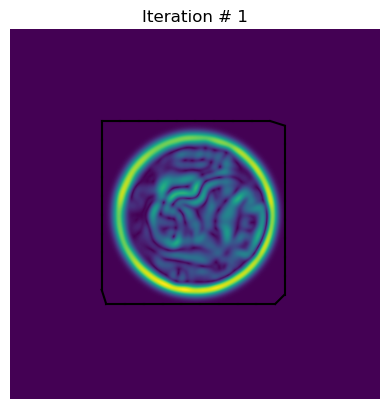
\includegraphics[width=0.18\textwidth]{it_1_no_shape.png}
    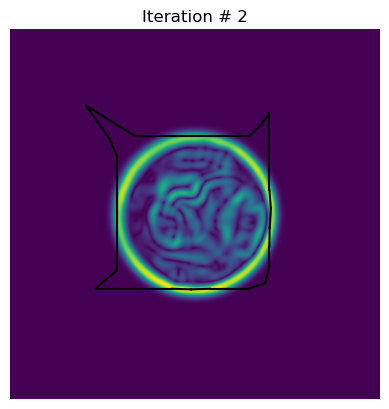
\includegraphics[width=0.18\textwidth]{it_2_no_shape.png}
      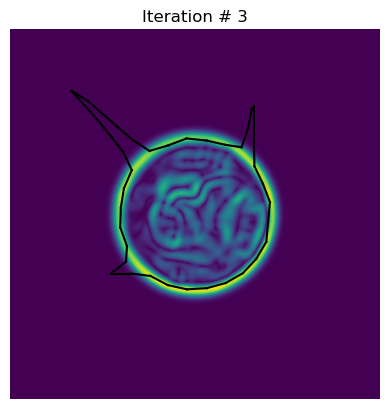
\includegraphics[width=0.18\textwidth]{it_3_no_shape.png}
        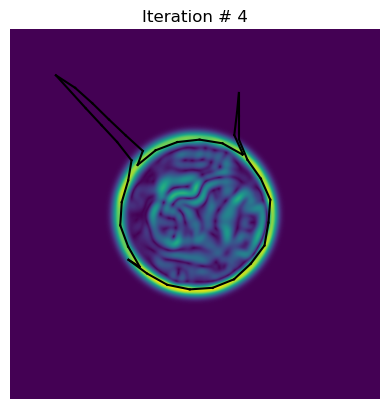
\includegraphics[width=0.18\textwidth]{it_4_no_shape.png}
          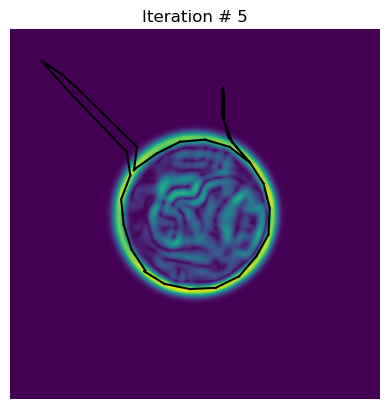
\includegraphics[width=0.18\textwidth]{it_5_no_shape.png}
  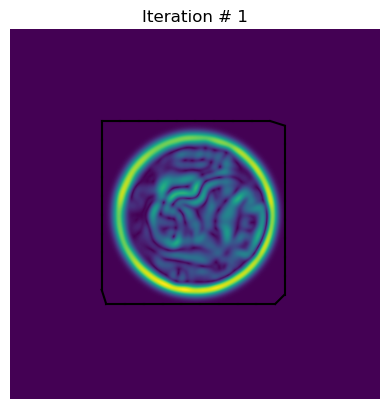
\includegraphics[width=0.18\textwidth]{it_1_alph_10_bet_0.png}
    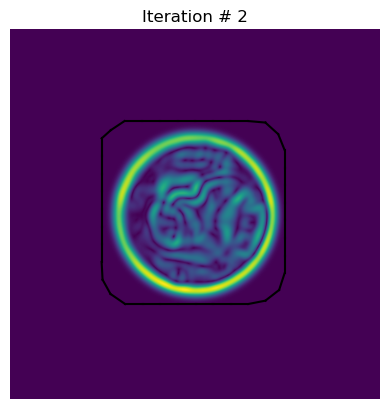
\includegraphics[width=0.18\textwidth]{it_2_alph_10_bet_0.png}
      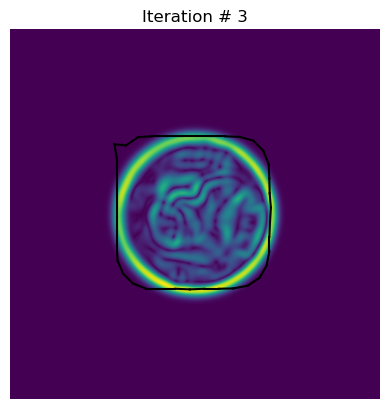
\includegraphics[width=0.18\textwidth]{it_3_alph_10_bet_0.png}
        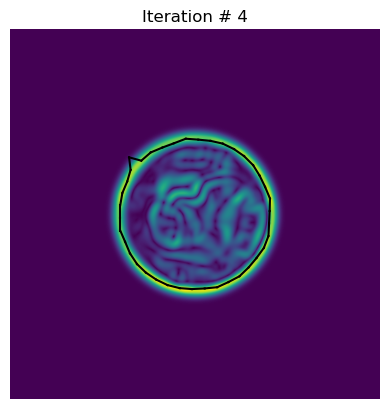
\includegraphics[width=0.18\textwidth]{it_4_alph_10_bet_0.png}
          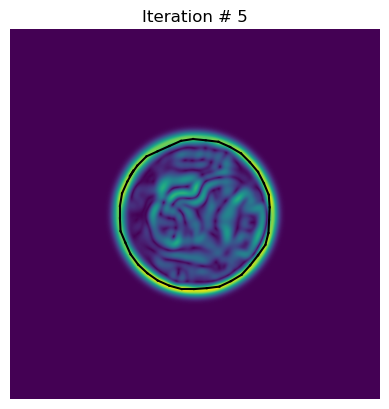
\includegraphics[width=0.18\textwidth]{it_5_alph_10_bet_0.png}          
  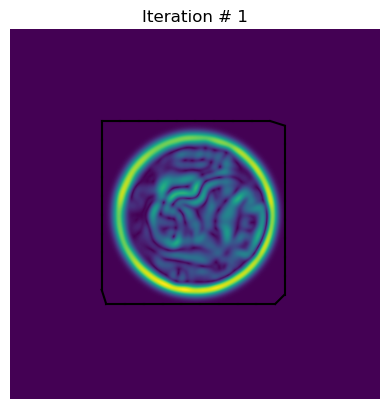
\includegraphics[width=0.18\textwidth]{it_1_alph_0_bet_10.png}
    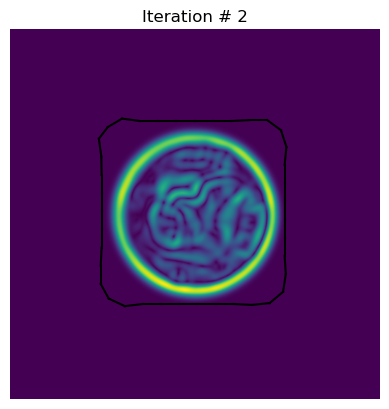
\includegraphics[width=0.18\textwidth]{it_2_alph_0_bet_10.png}
      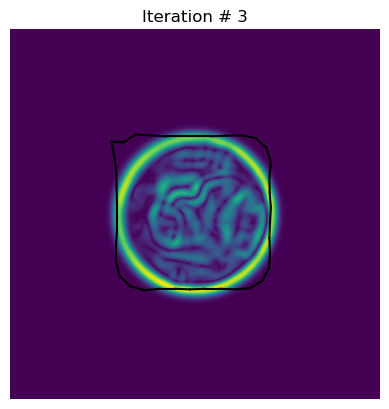
\includegraphics[width=0.18\textwidth]{it_3_alph_0_bet_10.png}
        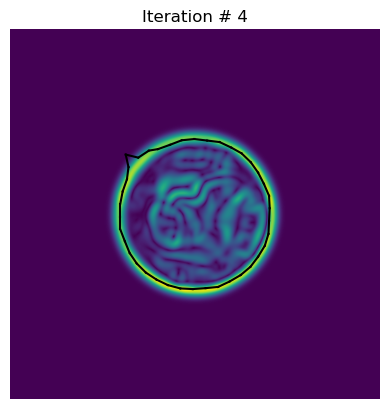
\includegraphics[width=0.18\textwidth]{it_4_alph_0_bet_10.png}
          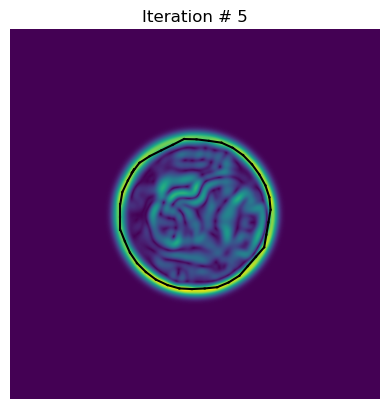
\includegraphics[width=0.18\textwidth]{it_5_alph_0_bet_10.png}
          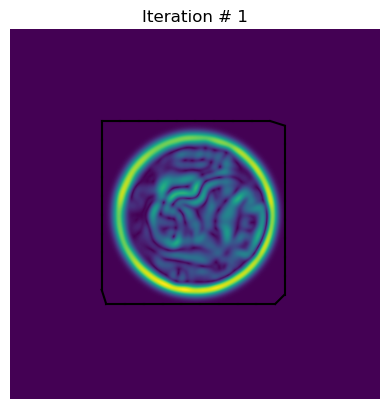
\includegraphics[width=0.18\textwidth]{it_1_alph_0_bet_10_min7.png}
    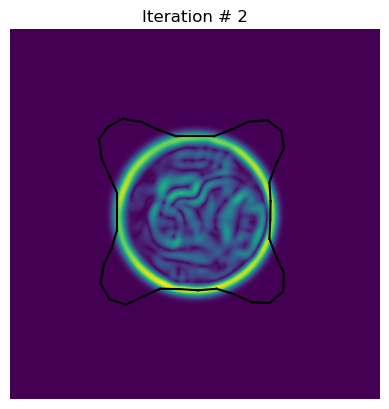
\includegraphics[width=0.18\textwidth]{it_2_alph_0_bet_10_min7.png}
      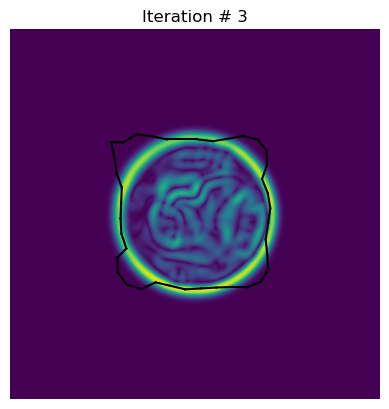
\includegraphics[width=0.18\textwidth]{it_3_alph_0_bet_10_min7.png}
        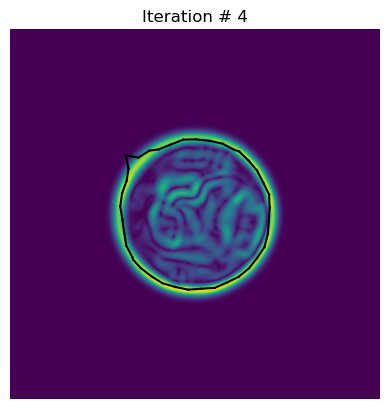
\includegraphics[width=0.18\textwidth]{it_4_alph_0_bet_10_min7.png}
          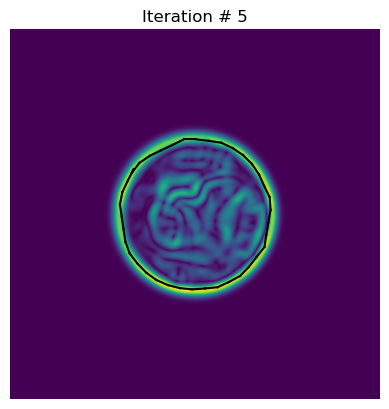
\includegraphics[width=0.18\textwidth]{it_5_alph_0_bet_10_min7.png}          
  \caption{For the four simulations, 40 control points were used, and a half window size of 50 pixels, First row: $\alpha= \beta = 0$, Second row: $\alpha= 10, \beta = 0$, 
  Third row: $\alpha= 0, \beta = 10$ . Fourth row: $\alpha= 0, \beta = 10^{-7}$}, 
  \label{fig:snake_results}
\end{figure}

\begin{figure}[h!]

\includegraphics[width=0.18\textwidth]{Rugby_im.png}
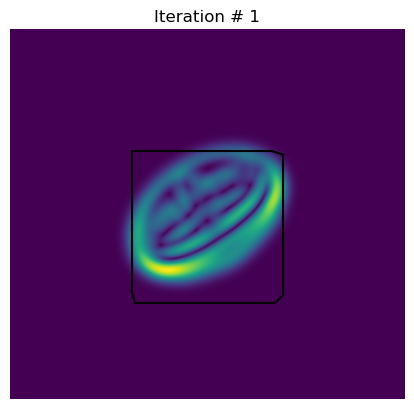
\includegraphics[width=0.18\textwidth]{Rugby_it_1.png}
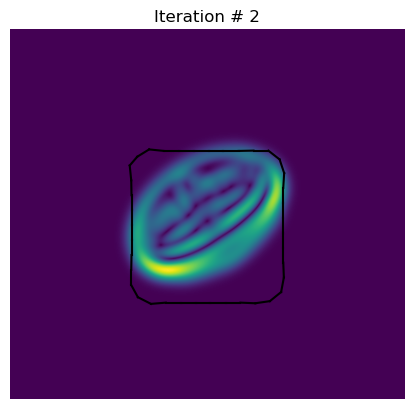
\includegraphics[width=0.18\textwidth]{Rugby_it_2.png}
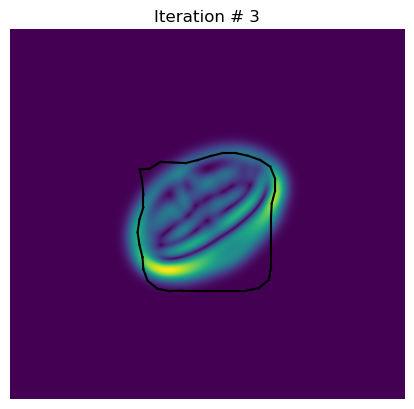
\includegraphics[width=0.18\textwidth]{Rugby_it_3.png}
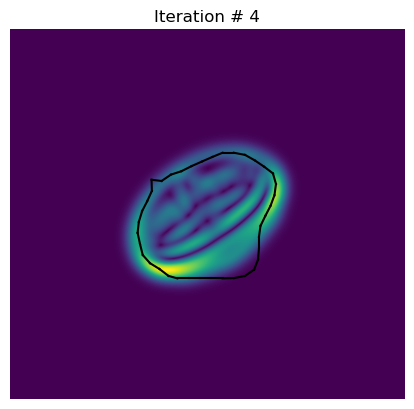
\includegraphics[width=0.18\textwidth]{Rugby_it_4.png}
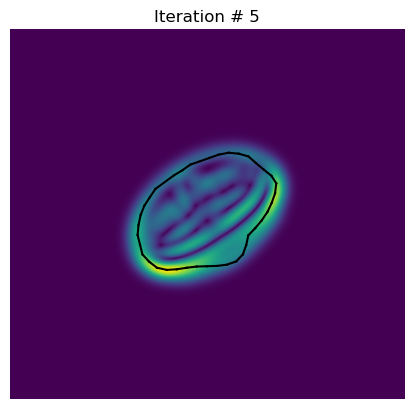
\includegraphics[width=0.18\textwidth]{Rugby_it_5.png}
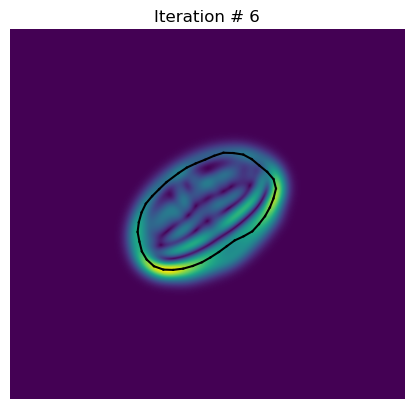
\includegraphics[width=0.18\textwidth]{Rugby_it_6.png}
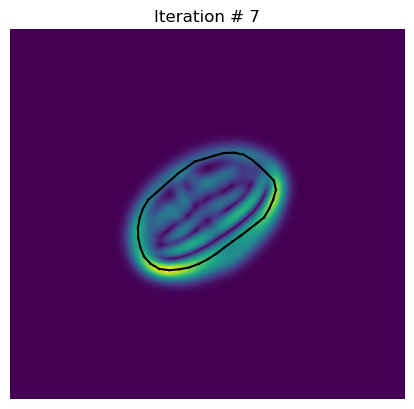
\includegraphics[width=0.18\textwidth]{Rugby_it_7.png}
\caption{40 control points were used, and a half window size of 40 pixels, First row: $\alpha= \beta = 10$}
\label{fig:snake_resultsv2}
\end{figure}

%\caption{ggg}

%    \includegraphics[width=0.18\textwidth{Rugby_it_2.png}
%    \includegraphics[width=0.18\textwidth{Rugby_it_3.png}
%    \includegraphics[width=0.18\textwidth{Rugby_it_4.png}            



\section{Conclusion}

In this report I went into the details of what are Snakes, how do they work, and provided an implementation of them.

Some of the known limitations of the snakes include: sensitivity to initialization, local minima, computational cost, and sensitivity to noise and intensity variations. 

One can use matematical morphology operations, like thresholding, dilation, skeletonize  and subsampling to initialize the snake. 




In spite of the advent of more recent techniques based on deep learning, snakes are still used in computer vision and in particular in medical imaging, due to their capacity to adapt to complex shapes and to their flexibility (ie the possibility to use different energy terms, see \citep{Snake}).


%\bibliographystyle{unsrtnat}
%\bibliography{references}


\bibliographystyle{plain}
\bibliography{references}



\end{document}


